% Part: history
% Chapter: set-theory
% Section: limits

\documentclass[../../../include/open-logic-section]{subfiles}

\begin{document}
	
\olfileid{his}{set}{limits}	

\olsection{લક્ષની ચુસ્ત વ્યાખ્યા}
	
આજે અગાઉની સમસ્યાનો પ્રમાણભૂત ઉકેલ
અનંતસૂક્ષ્મોને દૂર કરવાનો છે. તે કેવી રીતે થાય છે તે જોઈએ.

આપણે જોયું કે $\beta$ નાનું થાય તેમ ઢાળના વધુ સારા
અંદાજ મળે છે. ખરેખર $\beta$ ગમે તેટલું
$0$ની નજીક જાય તેમ $f'(c)$ માટેનો અંદાજ
આપણે ઇચ્છતા ઢાળ તરફ જાય છે. તેથી
$\beta = 0$ \emph{પર} શું થાય છે તે
જોવાને બદલે, $\beta$ જ્યારે $0$ની નજીક
જાય ત્યારે $f'(c)$ માટેના અંદાજનું
\emph{વલણ} જોવું પૂરતું છે.

આ રીતે કહીએ તો સામાન્ય પડકાર નીચેના પ્રકારના
વિધાનનો અર્થ સ્પષ્ટ કરવાનો છે:
\begin{center}
$x$ જ્યારે $c$ની નજીક જાય, ત્યારે $g(x)$
$\ell$ તરફ જાય છે.
\end{center}
આને વધુ સંક્ષેપમાં આમ લખી શકાય:
\[
\lim_{x \rightarrow c}g(x) = \ell.
\]
ઓગણીસમી સદીમાં કોશીના અગાઉના કાર્યના આધારે
વાયરસ્ટ્રાસે આ નિરૂપણની સંપૂર્ણ ચુસ્ત વ્યાખ્યા
આપી. વિચાર એ છે કે $x$ને~$c$ની
યોગ્ય રીતે નજીક લઈ જઈએ તો $g(x)$ને
ઇચ્છીએ તેટલું~$\ell$ની નજીક લાવી શકીએ.
વધુ ચોક્કસ રીતે,
$\lim_{x \rightarrow c} g(x) = \ell$
નો અર્થ નીચે મુજબ નક્કી કરીએ:
\[
(\forall\epsilon > 0)(\exists \delta > 0)\forall x \left(0<|x - c| < \delta \lif |g(x) - \ell| < \epsilon \right).
\]
\sourcecorrection{OLMD-167}{મૂળ પાઠમાં આ લક્ષની
વ્યાખ્યાની પૂર્વશરતમાં $0<|x-c|$ છૂટી ગયું છે.
એ શરત વિના $x=c$ પણ લેવાય અને $g(c)$
અલગ હોય ત્યારે સાચું લક્ષ ખોટું ઠરે.
ઉપર અગાઉનો $f'(c)$ પોતે બદલાય છે એવો
ઉલ્લેખ પણ ચોક્કસ નથી; બદલાતો ભાગાકાર
તેના મૂલ્યનો અંદાજ આપે છે.}
અહીં ઊભી રેખાઓ નિરપેક્ષ મૂલ્ય દર્શાવે છે.
અર્થાત્ $x \geq 0$ હોય ત્યારે $|x| = x$
અને $x < 0$ હોય ત્યારે $|x| =-x$;
આ \emph{વિધેય}નું ચિત્ર આ પ્રમાણે છે:
\begin{center}
	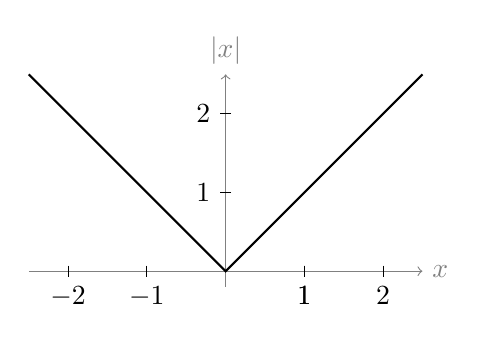
\begin{tikzpicture}[scale=1]
	\draw[->, gray] (-2.5,0) -- (2.5,0) node[right] {$x$};
	\draw[->, gray] (0,-.2) -- (0,2.5) node[above] {$|x|$};
	
	\foreach \x/\xtext in {-2/-2, -1,1, 1/1, 2/2}
	\draw[shift={(\x,0)}] (0pt,2pt) -- (0pt,-2pt) node[below] {{$\xtext$}};
	
	\foreach \y/\ytext in {1/1, 2/2}
	\draw[shift={(0,\y)}] (2pt,0pt) -- (-2pt,0pt) node[left] {{$\ytext$}};
	
	\draw[thick] (-2.5, 2.5)--(0,0)--(2.5, 2.5);
	\end{tikzpicture}
\end{center}
આ વ્યાખ્યા આશરે એમ કહે છે કે~$c$થી
$\delta$ કરતાં ઓછા અંતરે આવેલા
નિવેશો પસંદ કરીને (અર્થાત્ $|x -
c| < \delta$), “ભૂલ”ને
$\epsilon$ કરતાં ઓછી કરી શકાય
(અર્થાત્ $|g(x) - \ell| < \epsilon$).

લક્ષની કલ્પના વ્યાખ્યાયિત કર્યા પછી
અનંતસૂક્ષ્મો વિના જ આગળ વધી શકીએ:
$c$ પર $f$નો ઢાળ આ પ્રમાણે નક્કી કરીએ:
\[
	{f}'(c) = \lim_{x \rightarrow 0}\left(\frac{f(c +x) - f(c)}{x}\right) \text{ જ્યાં લક્ષ અસ્તિત્વમાં હોય}.
\]
પરંતુ વ્યાખ્યામાં “જ્યાં લક્ષ અસ્તિત્વમાં હોય”
એ શરત શા માટે જરૂરી છે તે સમજવું મહત્વનું છે.
હમણાં ચિત્રમાં જોયેલું $f(x) = |x|$
સરળ ઉદાહરણ છે. સ્પષ્ટ છે કે $f'(0)$
સુવ્યાખ્યાયિત નથી: $0$ની “જમણી બાજુથી”
નજીક જઈએ તો ઢાળ હંમેશાં $1$ છે;
$0$ની “ડાબી બાજુથી” જઈએ તો ઢાળ
હંમેશાં $-1$ છે. તેથી લક્ષ અસ્તિત્વમાં
નથી. આથી વિધેય~$f$ બિંદુ~$x$ પર
ત્યારે અને ત્યારે જ \emph{વિકલનીય}
છે જ્યારે આવું લક્ષ અસ્તિત્વમાં હોય.

આપણે જોયું કે \emph{લક્ષ}ની કલ્પનાથી
વિકલનને કેવી રીતે સંભાળી શકાય.
એ જ કલ્પનાથી \emph{સતત} વિધેયનો
ખ્યાલ પણ વ્યાખ્યાયિત કરી શકીએ.
(બોલ્ઝાનોએ 1817 સુધીમાં આ વાતનો
મૂળ વિચાર સમજી લીધો હતો.)
સાતત્ય અંગે કોશી--વાયરસ્ટ્રાસનો
અભિગમ આ પ્રમાણે છે. આશરે કહીએ તો,
વિધેય~$f$ કોઈ બિંદુએ સતત ત્યારે છે
જ્યારે તેના નિર્ગમની ચોકસાઈ અંગેની
કોઈ માંગ તેના નિવેશની ચોકસાઈ
નક્કી કરીને પૂરી કરી શકાય.
વધુ ચોક્કસ રીતે, $f$ બિંદુ $c$
પર સતત છે જો $x$ શૂન્ય તરફ
જાય ત્યારે $f(c + x)$ અને $f(c)$
વચ્ચેનો તફાવત પણ $0$ તરફ જાય.
બીજા શબ્દોમાં, $f$ બિંદુ $c$
પર ત્યારે અને ત્યારે જ
\emph{સતત} છે જ્યારે
$f(c) = \lim_{x \rightarrow c} f(x)$.

આગળ વધીએ તો આપણો વિષય ગણસિદ્ધાંતમાંથી
વાસ્તવિક વિશ્લેષણ તરફ વળી જશે. તેથી
અહીં અટકી આ ચર્ચાનો સાર કહીએ:
ઓગણીસમી સદીમાં ગણિતશાસ્ત્રીઓએ
\emph{લક્ષ}ની ચુસ્ત વ્યાખ્યાયિત કલ્પનાથી
અનંતસૂક્ષ્મો વિના કામ કરવાનું શીખ્યું.

\end{document}
